\documentclass[11pt]{article}
\usepackage[T1]{fontenc}
\usepackage{lmodern}
\usepackage[margin=0.9in]{geometry}
\usepackage{amsmath,amssymb,amsthm}
\usepackage{microtype}
\usepackage{graphicx}
\usepackage{booktabs}
\usepackage{placeins}
\usepackage[colorlinks=true,linkcolor=blue,citecolor=blue,urlcolor=blue]{hyperref}
\hypersetup{
  pdftitle={Parity Rock-Paper-Scissors Games and the Alper Constant},
  pdfauthor={Alper Ferudun},
  pdfsubject={Unrefereed mathematical preprint},
  pdfkeywords={Nash equilibrium, zero-sum game, asymptotic expansion, Alper constant}
}
\newtheorem{theorem}{Theorem}[section]
\newtheorem{lemma}[theorem]{Lemma}
\newtheorem{corollary}[theorem]{Corollary}
\newtheorem{proposition}[theorem]{Proposition}
\newtheorem*{theoremA}{Theorem A}
\newtheorem*{theoremB}{Theorem B}
\theoremstyle{definition}
\newtheorem{definition}[theorem]{Definition}
\newtheorem{example}[theorem]{Example}
\theoremstyle{remark}
\newtheorem{remark}[theorem]{Remark}
\DeclareMathOperator{\sgn}{sgn}
\newcommand{\E}{\mathbb{E}}
\newcommand{\Alp}{\mathcal{A}}
\newcommand{\Hodd}{H^{\mathrm{odd}}}
\title{Parity Rock--Paper--Scissors Games\\and the Alper Constant}
\author{Alper Ferudun\thanks{Mercury Software GmbH.
Email: \href{mailto:alper@mercurycodelab.com}{alper@mercurycodelab.com}.
GitHub: \href{https://github.com/AlperTheKing}{AlperTheKing}.}}
\date{5 October 2026}
\begin{document}
\maketitle

\begin{abstract}
Two players choose numbers from $\{1,\dots,n\}$. Equal numbers draw, an
odd difference is won by the smaller number, a nonzero even difference is
won by the larger number, and a win with the number $m$ pays $2m-h$, where
$0\le h<2$ is fixed. For $h=1$ this is the game of Problem~1012 of
Project Euler; for $h=0$ the payment is proportional to the winning
number. For every $h$ outside an explicit countable set we prove that the
game has a unique equilibrium, supported on $2k+1$ consecutive numbers
ending at $n$ or $n-1$, and we solve it in closed form. When the support
ends at $n$, the probability $P(n)$ of the largest number is
$\bigl((2k^2+1)R_k-2(k^2-1)\bigr)/\bigl(3(2k+1)\bigr)$ for an explicit
product $R_k$ that depends only on the largest payment; otherwise $P(n)=0$.
The support
widens at thresholds given by the zeros of these functions; for
$h\in\{0,1\}$ the thresholds are cubic polynomials in $k$ for each parity. For
$S_h(N)=\sum_{n=3}^{N}P(n)$ and $h\in\{0,1\}$ we prove
$S_h(N)=(3/2)^{4/3}N^{1/3}-\tfrac14\log N-\Alp(h)-\tfrac32\tau(1-\tau)
+O(N^{-1/3})$, where $\tau\in[0,1)$ is the relative position of $N$ in its
block, and we determine the next term. The constant $\Alp(h)$ plays the
role that Euler's constant plays for the harmonic series. We call
$\Alp=\Alp(0)=1.7771799879\ldots$ the Alper constant, give a series and
an integral representation, and certify $80$ decimal places of $\Alp$ and
of $\Alp(1)=1.6464176534\ldots$ with interval arithmetic. No expression
of either constant in classical constants was found.
\end{abstract}

\section{Introduction}

In rock--paper--scissors every option beats exactly one other option.
With equal payments the unique equilibrium is uniform. Unequal payments
change the picture in a counterintuitive way. Suppose the loser pays $5$
to a winning rock, $3$ to a winning paper and $1$ to winning scissors.
Then the unique equilibrium plays rock, paper and scissors with
probabilities $\frac19$, $\frac59$ and $\frac13$: the most lucrative
option is used least.

We study the following family of extensions to $n$ options. Two players
choose numbers from $\{1,\dots,n\}$ simultaneously. Equal numbers draw. If
the numbers differ by an odd amount, the smaller number wins. If they
differ by a nonzero even amount, the larger number wins. A win with the
number $m$ is paid $2m-h$ by the loser, where $0\le h<2$ is a fixed
parameter. We write $G_n(h)$ for this game. Every increasing payment
schedule $c\,(m-\theta)$ with $c>0$ and $0\le\theta<1$ is covered after
scaling, with $h=2\theta$. Two members stand out:
\begin{itemize}
\item $h=1$: the payments are $1,3,5,\dots$. For $n=3$ the numbers
$1,2,3$ play the roles of scissors, paper and rock with the payments
$1,3,5$ above. This game was posed as Problem~1012 of Project
Euler~\cite{PE}, and a solution is described in~\cite{ES}.
\item $h=0$: the payment is proportional to the winning number. This is
the simplest member, and the one whose constant we call the Alper
constant.
\end{itemize}
Whenever the equilibrium is unique, let $P(n)$ be the probability that
it assigns to the largest number $n$, and put
\[
S_h(N)=\sum_{n=3}^{N}P(n).
\]
In particular, these quantities are unambiguous for $h\notin\mathcal E$,
where the exceptional set $\mathcal E$ is defined below.

Solving $G_n(h)$ numerically for moderate $n$ and generic $h$ suggests
that the equilibrium plays an odd number of consecutive numbers and
that its width grows by two at isolated values of $n$. Sampled ratios
$S_0(N)/N^{1/3}$ approach their limit slowly: the ratio is $1.330$ at $N=10^3$ and
$1.613$ at $N=10^5$, while its limit turns out to be
$(3/2)^{4/3}\approx1.7171$. We prove the support and transition laws
for every $h\notin\mathcal E$, and the asymptotic formulas for
$h\in\{0,1\}$. The latter isolate the constant that governs the slow approach.

Throughout, $\log$ is the natural logarithm, $\gamma$ is Euler's
constant and $c_j=\binom{2j}{j}4^{-j}$. For $k\ge1$ and real $y$ put
\begin{equation}\label{eq:R-P}
R_k(y)=\prod_{j=1}^{k}\frac{y-2j}{y-2j+1},\qquad
P_k(y)=\frac{(2k^2+1)\,R_k(y)-2(k^2-1)}{3(2k+1)} .
\end{equation}
The variable $y$ will be half of the largest payment in play, so
$y=n-\frac h2$ when the largest number is $n$. For $k\ge2$ the function
$P_k$ increases on $y>2k$ and has exactly one zero $\beta_k$ there
(Lemma~\ref{lem:root}). Put $t_1(h)=3$ and $t_k(h)=\lfloor\beta_k+\frac
h2\rfloor+1$ for $k\ge2$: this is the first integer $n$ with
$P_k(n-\frac h2)>0$. The integers $n$ with $t_k(h)\le n\le t_{k+1}(h)-1$
form the \emph{block} $k$; the blocks partition the integers $n\ge3$.
Finally let $\mathcal E$ be the set of $h\in[0,2)$ for which
$\beta_k+\frac h2$ is an integer for some $k\ge2$. It is countable, and it
contains neither $0$ nor $1$.

\begin{theoremA}[Theorems~\ref{thm:interval} and~\ref{thm:structure}]
Let $0\le h<2$, $h\notin\mathcal E$, and $n\ge3$. The game $G_n(h)$ has a
unique equilibrium. Let $k$ be the block of $n$. If $n\le t_{k+1}(h)-2$,
the support is $\{n-2k,\dots,n\}$ and $P(n)=P_k(n-\frac h2)>0$. If
$n=t_{k+1}(h)-1$, the support is $\{n-1-2k,\dots,n-1\}$ and $P(n)=0$.
The whole equilibrium is given in closed form by
Theorem~\ref{thm:interval}. For the two main cases
\[
t_k(0)=\Bigl\lceil\frac{4k^3+5k}{6}\Bigr\rceil+1,\qquad
t_k(1)=\Bigl\lfloor\frac{4k^3+5k}{6}\Bigr\rfloor+2 .
\]
\end{theoremA}

The first values are $t_k(0)=3,8,22,47,89,150,236,349$ and
$t_k(1)=3,9,22,48,89,151,236,350$.

\begin{theoremB}[Theorem~\ref{thm:asymptotics}]
Let $h\in\{0,1\}$ and $\kappa=(3/2)^{4/3}=\sqrt[3]{81/16}$. For $N\ge3$ let
$K$ be defined by $t_K(h)-1\le N<t_{K+1}(h)-1$, and put
$\tau=(N-t_K(h)+1)/(t_{K+1}(h)-t_K(h))\in[0,1)$. Then, uniformly in $\tau$,
\[
S_h(N)=\kappa N^{1/3}-\tfrac14\log N-\Alp(h)-\tfrac32\,\tau(1-\tau)
-\frac{1-3\tau(1-\tau)(4\tau-1)}{4K}+O\bigl(N^{-2/3}\bigr).
\]
\end{theoremB}

Since $K=(3N/2)^{1/3}+O(1)$, the term with $1/K$ is of order $N^{-1/3}$.
The quadratic term cannot be dropped: within every block,
$S_h(N)-\kappa N^{1/3}+\frac14\log N$ sweeps from about $-\Alp(h)$ down to
about $-\Alp(h)-\frac38$ and back. At the ends of the blocks, where $P$
vanishes and $\tau=0$, the oscillation disappears.

\emph{The Alper constant.} The constant $\Alp(h)$ is an Euler-type
constant. The harmonic numbers satisfy
$H_N-\log N\to\gamma$; here, along the ends $N_K=t_{K+1}(h)-1$ of the
blocks,
\[
\kappa N_K^{1/3}-\tfrac14\log N_K-S_h(N_K)\longrightarrow\Alp(h)
\qquad(K\to\infty).
\]
We define the \emph{Alper constant} as the constant of the simplest
member, $h=0$:
\[
\begin{aligned}
\Alp=\Alp(0)\approx1.&7771799879054231885280182162763415624255\\
&7103207026437429288159344562194194456353
\end{aligned}
\]
For the Project Euler game,
\[
\begin{aligned}
\Alp(1)\approx1.&6464176534405600338544841159858132863029\\
&9683869991753007336025510008825020074857
\end{aligned}
\]
Section~\ref{sec:constant} expresses both constants as rapidly computable
series and as integral-series, and certifies that the values above are
correctly rounded to $80$ decimal places.

The case $h=1$ is a Project Euler problem, and its solvers may have
obtained parts of our results for it, including the closed form and the
first-order asymptotic formula; we make no priority claim for this case.
The contributions developed here include the family $G_n(h)$, its
transition law for general $h$, proofs of the asymptotic formulas for
$h\in\{0,1\}$, the second-order term, the Alper constant and the
certified digits. Section~\ref{sec:game}
sets up the games, Section~\ref{sec:support} shows that the supports are
intervals, and Section~\ref{sec:interval} solves the equilibrium
equations on an interval of odd length. Section~\ref{sec:structure}
proves the transition law and Theorem~A. Section~\ref{sec:blocks} sums the
probabilities over blocks. Section~\ref{sec:asymptotics} proves
Theorem~B, Section~\ref{sec:constant} studies the constants, and
Section~\ref{sec:numerics} compares the theorems with exact values of
$S_0(10^m)$ for $m\le20$.

\section{The games}\label{sec:game}

Let $a_{ij}$ be the payment received by a player who chooses $i$ when the
opponent chooses $j$. It is $0$ for $i=j$. Otherwise the winning number
$w$ is $\min(i,j)$ when $i-j$ is odd and $\max(i,j)$ when $i-j$ is even,
and the winner receives $2w-h$.

\begin{lemma}\label{lem:payoff}
For all $i,j$,
$a_{ij}=(i-j)+\sgn(i-j)\,(-1)^{i+j}\,(i+j-h)$. In particular
$a_{ji}=-a_{ij}$.
\end{lemma}

\begin{proof}
Take $j<i$. If $i-j$ is even, $i$ wins and the formula gives
$(i-j)+(i+j-h)=2i-h$. If $i-j$ is odd, $j$ wins and it gives
$(i-j)-(i+j-h)=-(2j-h)$. The case $j>i$ follows by antisymmetry.
\end{proof}

Against a vector $p=(p_1,\dots,p_n)$ the pure option $i$ earns
$f_i=\sum_{j}a_{ij}p_j$, and we use this formula for every integer $i$.
Since $A=(a_{ij})$ is skew-symmetric, $p^{\mathsf T}Ap=0$, and the value of
the game is $0$. Hence a probability vector $p$ is an equilibrium exactly
when
\begin{equation}\label{eq:eq-conditions}
p_i\ge0,\qquad \sum_ip_i=1,\qquad f_i\le0\ \text{for all } i,\qquad
f_i=0\ \text{whenever } p_i>0;
\end{equation}
the last condition follows from the others because
$\sum_ip_if_i=p^{\mathsf T}Ap=0$. An equilibrium exists for every $n$ by
the minimax theorem~\cite{vN}. The payoff rule does not depend on $n$, so
the matrix of $G_{n-1}(h)$ is a principal submatrix of the matrix of
$G_n(h)$.

For $n=3$ the payoffs are $f_1=(2-h)p_2-(6-h)p_3$,
$f_2=-(2-h)p_1+(4-h)p_3$ and $f_3=(6-h)p_1-(4-h)p_2$. Setting them to
zero and normalising gives
\[
p=\frac{(4-h,\;6-h,\;2-h)}{12-3h},
\]
so $p=(\frac13,\frac12,\frac16)$ for $h=0$ and
$p=(\frac13,\frac59,\frac19)$ for $h=1$, the weighted
rock--paper--scissors equilibrium of the introduction.

\section{Interval supports}\label{sec:support}

For a probability vector $p$ let $X_i$ be the probability that option
$i$ wins: the total mass of the numbers $j<i$ of the parity of $i$ and of
the numbers $j>i$ of the other parity.

\begin{lemma}\label{lem:rows}
For every probability vector $p$ and every $i\le n-2$,
\[
f_{i+2}-f_i=4\bigl(X_i-p_{i+1}\bigr)+(2i+4-h)\bigl(p_i+p_{i+2}\bigr)
-(4i+2-2h)\,p_{i+1},\qquad X_i\ge p_{i+1}.
\]
\end{lemma}

\begin{proof}
The options $i$ and $i+2$ have the same parity, so they obtain the same
result against every $j\notin\{i,i+1,i+2\}$. When both win, $i+2$
receives $4$ more. The three remaining columns give
$a_{i+2,i}-a_{ii}=2i+4-h$,
$a_{i+2,i+1}-a_{i,i+1}=-(2i+2-h)-(2i-h)=-(4i+2-2h)$ and
$a_{i+2,i+2}-a_{i,i+2}=2i+4-h$. Option $i$ beats $i+1$, which gives
$X_i\ge p_{i+1}$.
\end{proof}

\begin{proposition}\label{prop:support}
Let $n\ge3$ and let $p$ be an equilibrium of $G_n(h)$. Its support is an
interval $\{a,\dots,b\}$ with $b\in\{n-1,n\}$ and $b>a$.
\end{proposition}

\begin{proof}
Suppose $p_i>0$ and $p_{i+1}=0$ for some $i\le n-2$. Then $f_i=0$ and
Lemma~\ref{lem:rows} gives $f_{i+2}\ge(2i+4-h)p_i>0$, which
contradicts~\eqref{eq:eq-conditions}. So every chosen number below $n-1$
is followed by another chosen number, and the support is an interval
$\{a,\dots,b\}$ with $b\ge n-1\ge2$. A single number $b\ge2$ is not an
equilibrium, because $b-1$ beats it and receives $2b-2-h>0$.
\end{proof}

For $h\notin\mathcal E$ the support has odd size, as proved in
Proposition~\ref{prop:odd}.
For the payments $1,3,5,\dots$ of $h=1$ there is a short argument modulo
$2$, but for general nonexceptional $h$ the parity of the support follows
from the explicit solution of the next section.

\section{The equilibrium on an interval of odd length}\label{sec:interval}

Fix $k\ge1$, $b\ge2k+1$, $a=b-2k$, $L=2k+1$, $I=\{a,\dots,b\}$ and
$y=b-\frac h2$, so that $2y$ is the payment for a win with $b$. For a
real vector $p$ supported on $I$ put
\[
s=\sum_jp_j,\qquad M=\sum_jj\,p_j,\qquad q_i=\sum_{j\le i}(-1)^{i-j}p_j\
\ (i\in\mathbb Z),\qquad Q=q_b .
\]
Thus $q_i=0$ for $i<a$, $q_i=(-1)^{i-b}Q$ for $i\ge b$, and
$p_i=q_i+q_{i-1}$. The numbers of the parity of $b$ carry the mass
$\frac{s+Q}2$, and the others carry $\frac{s-Q}2$.

\begin{lemma}[moment equation]\label{lem:moment}
For $a\le j\le b$,
\[
\sum_{i=a}^{b}a_{ij}=L\Bigl(\frac{a+b}2-j\Bigr)+
\begin{cases}k,&j\equiv b\pmod2,\\-(k+1),&j\not\equiv b\pmod 2,\end{cases}
\]
independently of $h$. Consequently, if $f_i=0$ for all $i\in I$, then
$L\bigl(\frac{a+b}2s-M\bigr)+k\frac{s+Q}2-(k+1)\frac{s-Q}2=0$; for $s=1$
this reads $M-\frac Q2=\frac{a+b}2-\frac1{2L}$, and for $s=0$ it reads
$M=\frac Q2$.
\end{lemma}

\begin{proof}
The column sum follows from Lemma~\ref{lem:payoff} by pairing
consecutive terms; the terms containing $h$ cancel. Adding the $L$
equations $f_i=0$ gives the stated equation.
\end{proof}

\begin{lemma}[neighbour identity]\label{lem:neighbour}
For every real vector $p$ supported on $I$ and every integer $i$,
\[
f_i+f_{i+1}=(2i+1)\,s-2M+(-1)^{b-i}Q+(2i+2-h)\,q_{i+1}-(2i-h)\,q_{i-1}.
\]
\end{lemma}

\begin{proof}
With $\varepsilon_j=(-1)^j$, Lemma~\ref{lem:payoff} gives
$f_i=is-M+\varepsilon_i\bigl[(i-h)T_i+U_i\bigr]$, where
$T_i=\sum_{j<i}\varepsilon_jp_j-\sum_{j>i}\varepsilon_jp_j$ and
$U_i=\sum_{j<i}\varepsilon_j\,j\,p_j-\sum_{j>i}\varepsilon_j\,j\,p_j$.
Passing from $i$ to $i+1$ changes $T_i$ and $U_i$ only in the terms of
$p_i$ and $p_{i+1}$, and $\varepsilon_{i+1}=-\varepsilon_i$, so
$f_i+f_{i+1}=(2i+1)s-2M-\varepsilon_iT_i-(2i+1-h)\,p_i+(2i+2-h)\,p_{i+1}$.
Finally $\varepsilon_iT_i=q_i-q_{i-1}-(-1)^{b-i}Q$, and
$p_i=q_i+q_{i-1}$, $p_{i+1}=q_{i+1}+q_i$.
\end{proof}

If $s=1$ and $f_i=0$ on $I$, the identity for $a\le i\le b-1$ gives the
$2k$ \emph{neighbour equations}
\begin{equation}\label{eq:neighbour}
(2i+2-h)\,q_{i+1}-(2i-h)\,q_{i-1}=2M-(2i+1)-(-1)^{b-i}Q
\qquad(a\le i\le b-1).
\end{equation}
Each equation links $q_{i-1}$ and $q_{i+1}$. The unknowns therefore split
into the chain $a-1,a+1,\dots,b-1$ and the chain $a,a+2,\dots,b$.

\begin{theorem}\label{thm:interval}
Let $p$ be a real vector supported on $I$ with $\sum_jp_j=1$ and $f_i=0$
for all $i\in I$. Put $R=R_k(y)$, $c_h=\frac{1-h}3$ and
\[
K=\frac{a+b-1}2-\frac1{2L},\qquad
Q=\frac{2y\,(R-1)+2k}3+\frac1L .
\]
Then $p_m=q_m+q_{m-1}$ with
\begin{align}
q_m&=K+c_h-\frac m3-\Bigl(K+c_h-\frac{a-1}3\Bigr)
\prod_{\substack{a\le i\le m-1\\ i\equiv b\ (2)}}\frac{2i-h}{2i+2-h}
&&(m=a-1,a+1,\dots,b-1),\label{eq:chain1}\\
q_m&=K+c_h+Q-\frac m3+\Bigl(\frac b3-K-c_h\Bigr)
\prod_{\substack{m+1\le i\le b-1\\ i\not\equiv b\ (2)}}\frac{2i+2-h}{2i-h}
&&(m=a,a+2,\dots,b).\label{eq:chain2}
\end{align}
In particular
\[
p_b=P_k(y),\qquad
p_a=K+c_h+Q-\frac a3+\Bigl(\frac b3-K-c_h\Bigr)\frac{y\,R}{y-2k}.
\]
\end{theorem}

\begin{proof}
On the first chain the equations~\eqref{eq:neighbour} have
$(-1)^{b-i}=1$. The homogeneous step multiplies by $\frac{2i-h}{2i+2-h}$.
A function $\gamma'-\frac m3$ is a particular solution exactly when
$2\gamma'=2M-1-Q+\frac{2-2h}3$, because
$(2i+2-h)(i+1)-(2i-h)(i-1)=6i+2-2h$. This gives
$\gamma'=M-\frac{1+Q}2+c_h=K+c_h$, by Lemma~\ref{lem:moment}. Starting
from $q_{a-1}=0$ gives~\eqref{eq:chain1}. Over the whole chain the
product is $R_k(y)$.

On the second chain $(-1)^{b-i}=-1$, the particular solution is
$K+c_h+Q-\frac m3$, and the chain ends at $q_b=Q$. Running it downwards
gives~\eqref{eq:chain2}. The full product over the second chain is
$1/R_k(y+1)$, and the telescoping identity
\begin{equation}\label{eq:telescope}
R_k(y)\,R_k(y+1)=\frac{y-2k}{y}
\end{equation}
gives the formula for $p_a=q_a$.

It remains to determine $Q$. Add the equations~\eqref{eq:neighbour}
for $a\le i\le b-1$:
\begin{itemize}
\item the left sides telescope to
$(2b-h)Q+(2b-2-h)q_{b-1}-(2a+2-h)q_a-2\sum_{m=a+1}^{b-2}q_m$;
\item the terms $\pm Q$ on the right cancel, and
$\sum_{i=a}^{b-1}(2i+1)=b^2-a^2$.
\end{itemize}
The normalisation $1=Q+2\sum_{m=a}^{b-1}q_m$ removes the remaining sum.
Together with Lemma~\ref{lem:moment} this yields
\begin{equation}\label{eq:endpoints}
2y\,p_b-(2a-h)\,p_a=(2k-1)\,Q+\frac1L,\qquad p_b=Q+q_{b-1}.
\end{equation}
Inserting the two chain solutions leaves a linear equation for $Q$ in
which $Q$ has the coefficient $L$. Its solution is the stated value.
Then $p_b=Q+q_{b-1}=P_k(y)$.
\end{proof}

\begin{lemma}[the kernel]\label{lem:kernel}
For every $0\le h<2$ the kernel of the principal submatrix $A_I$ is a
line, spanned by a vector with nonzero coordinate sum. Consequently the
formulas of Theorem~\ref{thm:interval} define a vector with
$\sum_jp_j=1$ and $f_i=0$ on $I$, and it is the only such vector.
\end{lemma}

\begin{proof}
A skew-symmetric matrix of odd order is singular, so $A_I$ has a nonzero
kernel vector $w$. Suppose that $\sum_jw_j=0$. Lemma~\ref{lem:moment}
gives $M=\frac Q2$, and Lemma~\ref{lem:neighbour} turns the equations
$f_i+f_{i+1}=0$, $a\le i\le b-1$, into
$(2i+2-h)q_{i+1}-(2i-h)q_{i-1}=2M-(-1)^{b-i}Q$. On the first chain the
right side is $0$, so $q\equiv0$ there, because $q_{a-1}=0$. On the
second chain the right side is $2Q$; the constant $Q$ is a solution, and
since $q_b=Q$ the solution is this constant. Hence $w_m=q_m+q_{m-1}=Q$
for all $m\in I$, so $0=\sum_jw_j=LQ$ and $w=0$, a contradiction. Thus
every nonzero kernel vector has nonzero sum and can be normalised;
Theorem~\ref{thm:interval} shows that the normalised kernel vector is
unique, so the kernel is a line.
\end{proof}

\begin{example}\label{ex:n10}
Take $h=0$, $b=10$ and $k=2$, so $I=\{6,\dots,10\}$, $y=10$ and
$R_2(10)=\frac89\cdot\frac67=\frac{16}{21}$. The theorem gives
\[
(p_6,p_7,p_8,p_9,p_{10})=\Bigl(\frac{29}{315},\frac{92}{315},
\frac{34}{105},\frac{74}{315},\frac{2}{35}\Bigr),
\]
with $Q=-\frac{17}{315}$ and $M=\frac{496}{63}$, so that
$M-\frac Q2=\frac{79}{10}=\frac{6+10}2-\frac1{10}$. This is the
equilibrium of $G_{10}(0)$, and $P(10)=\frac2{35}$.
\end{example}

\section{Neighbouring options and the transition law}\label{sec:structure}

The interval solution decides its own fate through the two options next
to the support.

\begin{proposition}\label{prop:neighbours}
In the setting of Theorem~\ref{thm:interval},
\[
f_{a-1}=\frac{2k+3}{2k+1}\,2y\,R_k(y)\,P_{k+1}(y+1),\qquad
f_{b+1}=-\frac{2k+3}{2k+1}\,(2y+2)\,P_{k+1}(y+2).
\]
\end{proposition}

\begin{proof}
Lemma~\ref{lem:neighbour} with $i=a-1$ (where $f_a=0$, $q_{a-2}=0$ and
$(-1)^{b-a+1}=-1$) and with $i=b$ (where $f_b=0$, $q_{b+1}=-Q$ and
$q_{b-1}=p_b-Q$) gives
\[
f_{a-1}=(2a-1)-2M-Q+(2a-h)\,p_a,\qquad
f_{b+1}=(2b+1)-2M-Q-2y\,p_b.
\]
By Lemma~\ref{lem:moment}, $2M+Q=a+b-\frac1L+2Q$, and
by~\eqref{eq:endpoints},
\[
f_{a-1}=2y\,p_b-L(1+Q),\qquad
f_{b+1}=L+\frac1L-2Q-2y\,p_b .
\]
Inserting $p_b=P_k(y)$ and the value of $Q$ from
Theorem~\ref{thm:interval}, both payoffs become affine in $R=R_k(y)$:
\begin{align*}
3L\,f_{a-1}&=(2k^2+4k+3)(2y-4k-2)-2k(k+2)\,2y\,R,\\
3L\,f_{b+1}&=2k(k+2)(2y+2)-(2k^2+4k+3)\,2y\,R.
\end{align*}
On the other hand, the definition of $R_{k+1}$ gives
\[
R_{k+1}(y+1)\,R_k(y)=\frac{y-2k-1}{y},\qquad
R_{k+1}(y+2)=\frac{y}{y+1}\,R_k(y).
\]
Since $2(k+1)^2+1=2k^2+4k+3$ and $2\bigl((k+1)^2-1\bigr)=2k(k+2)$, the
definition~\eqref{eq:R-P} of $P_{k+1}$ turns the right-hand sides into
$3(2k+3)\,2yR\,P_{k+1}(y+1)$ and $-3(2k+3)(2y+2)P_{k+1}(y+2)$.
\end{proof}

\begin{lemma}[root bound]\label{lem:root}
Let $k\ge2$. On the half-line $y>2k$ the function $P_k$ is continuous
and strictly increasing, and its unique zero $\beta_k$ satisfies
\[
\frac{4k^3+5k+3}{6}<\beta_k<\frac{4k^3+5k+6}{6}.
\]
In particular $\beta_k\notin\frac12\mathbb Z$. For $k=1$ we have
$P_1(y)=\frac{y-2}{3(y-1)}>0$ for $y>2$.
\end{lemma}

\begin{proof}
For $y>2k$ every factor of $R_k(y)$ is positive and increasing, so $R_k$
increases strictly from $0$ to $1$, and $P_k(y)=0$ exactly when
$-\log R_k(y)=\lambda_k:=\log\frac{2k^2+1}{2k^2-2}$. Put
$x=y-k-\frac12$ and
\[
U=\bigcup_{j=1}^{k}\bigl[k-2j+\tfrac12,\;k-2j+\tfrac32\bigr],\qquad
G(x)=\int_U\frac{dt}{x+t}.
\]
The interval with index $j$ contributes $\log\frac{y-2j+1}{y-2j}$, so
$G(x)=-\log R_k(y)$. The set $U$ is symmetric about $0$, has measure $k$
and lies in $[-d,d]$ with $d=k-\frac12$; on $x>d$ the function $G$ is
strictly decreasing. Let $x^*$ be the solution of $G(x^*)=\lambda_k$, so
that $\beta_k=x^*+k+\frac12$.

\emph{Lower bound.} Let $x_0=k(4k^2-1)/6>d$. Then
$x_0+\frac k2=\frac{k(2k^2+1)}3$ and $x_0-\frac k2=\frac{k(2k^2-2)}3$,
so $\int_{-k/2}^{k/2}\frac{dt}{x_0+t}=\lambda_k$. Folding both integrals
onto $t\ge0$ gives
\[
G(x_0)-\lambda_k=\int_{U_+}g(t)\,dt-\int_0^{k/2}g(t)\,dt,\qquad
g(t)=\frac{2x_0}{x_0^2-t^2},\quad U_+=U\cap[0,\infty).
\]
The set $U_+$ has measure $\frac k2$, and since $k\ge2$ it has positive
measure beyond $\frac k2$. As $g$ is strictly increasing on $[0,x_0)$,
the difference is positive. Hence $G(x_0)>\lambda_k$ and $x^*>x_0$.

\emph{Upper bound.} Let $z=x_0+\frac12$. By symmetry
$G(z)=\int_U\frac{z\,dt}{z^2-t^2}$, and for $|t|\le d$ we have
$\frac{z}{z^2-t^2}\le\frac1z\bigl(1+\frac{t^2}{z^2-d^2}\bigr)$. Since
$\int_Ut^2\,dt=kv$ with $v=\frac{4k^2-3}{12}$,
\[
G(z)\le\frac kz\Bigl(1+\frac{v}{z^2-d^2}\Bigr)<\frac k{x_0}.
\]
The second inequality is equivalent to $2x_0v<z^2-d^2=x_0^2+x_0-(k^2-k)$,
which follows from $x_0>2v$ and $x_0>k^2-k$. Finally
$\frac k{x_0}=\frac{6}{4k^2-1}=\frac{2u}{2+u}$ with $u=\frac3{2k^2-2}$,
and $\frac{2u}{2+u}<\log(1+u)=\lambda_k$. Hence $G(z)<\lambda_k$ and
$x^*<z$.

Thus $x_0<x^*<x_0+\frac12$, which is the stated bound because
$x_0+k+\frac12=\frac{4k^3+5k+3}6$. The number $\frac{4k^3+5k}6$ is an
integer for even $k$ and a half-integer for odd $k$, so the two bounds
are consecutive points of $\frac12\mathbb Z$.
\end{proof}

By Lemma~\ref{lem:root}, $t_k(h)=\lfloor\beta_k+\frac h2\rfloor+1$ is
the first integer $n$ with $P_k(n-\frac h2)>0$, and for $h\notin\mathcal
E$ no integer $n$ gives $P_k(n-\frac h2)=0$. Since
$\beta_k\notin\frac12\mathbb Z$, neither $0$ nor $1$ lies in $\mathcal
E$, and the bounds of Lemma~\ref{lem:root} give the formulas for
$t_k(0)$ and $t_k(1)$ stated in Theorem~A, equivalently
\begin{equation}\label{eq:tk-poly}
t_k(h)=\frac23k^3+\frac56k+\frac{5+2h-(-1)^{k+h}}4\qquad(h\in\{0,1\}).
\end{equation}

\begin{proposition}\label{prop:odd}
Let $h\notin\mathcal E$. Every equilibrium of $G_n(h)$ has a support of
odd size $2k+1\ge3$.
\end{proposition}

\begin{proof}
Suppose the support $I_0=\{a,\dots,b\}$ of an equilibrium $p$ has even
size $2k\ge2$, and let $I=\{a,\dots,b+1\}$; the option $b+1$ may lie
outside the game, and $f_{b+1}$ is computed with
Lemma~\ref{lem:payoff}. On $I$ we have $A_Ip=\varphi\,e_{b+1}$ with
$\varphi=f_{b+1}$, because $f_i=0$ on $I_0$. Let $v$ be the normalised
kernel vector of $A_I$ from Lemma~\ref{lem:kernel}. By
Theorem~\ref{thm:interval}, $v_{b+1}=P_k(b+1-\frac h2)$, which is
nonzero: for $k\ge2$ because $h\notin\mathcal E$, and for $k=1$ by
Lemma~\ref{lem:root}. Skew-symmetry gives
$0=-(A_Iv)^{\mathsf T}p=v^{\mathsf T}A_Ip=\varphi\,v_{b+1}$, so
$\varphi=0$. Then $p$ is a normalised kernel vector of $A_I$, so $p=v$
and $p_{b+1}=v_{b+1}\ne0$, a contradiction.
\end{proof}

\begin{theorem}\label{thm:structure}
Let $h\notin\mathcal E$ and let $n\ge3$ lie in the block $k$. The game
$G_n(h)$ has exactly one equilibrium. If $n\le t_{k+1}(h)-2$, its support
is $\{n-2k,\dots,n\}$ and $P(n)=P_k(n-\frac h2)>0$. If
$n=t_{k+1}(h)-1$, its support is $\{n-1-2k,\dots,n-1\}$ and $P(n)=0$.
\end{theorem}

\begin{proof}
Write $t_k$ for $t_k(h)$. Let $p$ be an equilibrium of $G_n(h)$; it
exists by the minimax theorem. By Propositions~\ref{prop:support}
and~\ref{prop:odd} its support is $\{a,\dots,b\}$ with $b\in\{n-1,n\}$
and $b-a=2k'$ for some $k'\ge1$, and by Theorem~\ref{thm:interval},
$p_b=P_{k'}(b-\frac h2)$.

First, $t_{k'}\le b\le t_{k'+1}-2$. Indeed $P_{k'}(b-\frac h2)=p_b>0$, so
$b\ge t_{k'}$. If $a\ge2$, the option $a-1$ exists and $f_{a-1}\le0$. As
$R_{k'}(b-\frac h2)>0$, Proposition~\ref{prop:neighbours} gives
$P_{k'+1}(b+1-\frac h2)\le0$, hence $<0$, and so $b+1<t_{k'+1}$. If
$a=1$, then $b=2k'+1\le t_{k'+1}-2$, because
$t_{k'+1}>\beta_{k'+1}>2k'+3$ by Lemma~\ref{lem:root}.

If $b=n-1$, the option $n=b+1$ exists and $f_n\le0$, so
$P_{k'+1}(b+2-\frac h2)\ge0$ by Proposition~\ref{prop:neighbours}, hence
$>0$, and $b+2\ge t_{k'+1}$. Together with the first step,
$n=t_{k'+1}-1$; this is the last element of the block $k'$, so $k'=k$,
$n=t_{k+1}-1$ and $P(n)=p_n=0$.

If $b=n$, the first step gives $t_{k'}\le n\le t_{k'+1}-2$, so $k'=k$,
$n\le t_{k+1}-2$ and $P(n)=p_n=P_k(n-\frac h2)>0$.

The two cases are distinguished by whether $n=t_{k+1}-1$, so the support
is determined by $n$. By Lemma~\ref{lem:kernel}, $p$ is the only
normalised vector on this support with vanishing payoffs on it. Hence the
equilibrium is unique.
\end{proof}

\begin{remark}\label{rem:exceptional}
The proof never checks that the closed-form probabilities are positive
or that the excluded options lose. Positivity and the sign conditions
are inherited from the equilibrium whose existence the minimax theorem
guarantees; as a by-product, every $p_m$ in Theorem~\ref{thm:interval}
is positive when $t_k(h)\le b\le t_{k+1}(h)-2$.

Write $\beta_k=\frac{4k^3+5k+3}6+\vartheta_k$ with
$0<\vartheta_k<\frac12$. Unwinding the definition of $t_k(h)$,
\[
\mathcal E=\{1-2\vartheta_k:\ k\ge2\text{ even}\}\cup
\{2-2\vartheta_k:\ k\ge3\text{ odd}\}.
\]
For even $k$, $t_k(h)$ equals $t_k(0)$ when $h<1-2\vartheta_k$ and
$t_k(1)$ when $h>1-2\vartheta_k$. For odd $k$, $t_k(0)=t_k(1)$, and
$t_k(h)$ equals this common value when $h<2-2\vartheta_k$ and exceeds it
by one when $h>2-2\vartheta_k$. In fact,
\[
\vartheta_k=\frac3{8k}+O(k^{-3}).
\]
To prove this, retain $U$, $G$ and $x_0=k(4k^2-1)/6$ from the proof of
Lemma~\ref{lem:root}, and put $V=[-k/2,k/2]$. Then
$\lambda_k=\int_V(x_0+t)^{-1}\,dt$. Both sets are symmetric, have
measure $k$ and lie in $[-k,k]$. Expanding the integrands, with the
odd moments cancelling, gives
\[
G(x_0)-\lambda_k
=\frac{\int_Ut^2\,dt-\int_Vt^2\,dt}{x_0^3}
  +O\!\left(\frac{k^5}{x_0^5}\right)
=\frac{k(k^2-1)}{4x_0^3}+O\!\left(\frac{k^5}{x_0^5}\right).
\]
Here $\int_Ut^2\,dt=k(4k^2-3)/12$ and $\int_Vt^2\,dt=k^3/12$.
Uniformly for $x_0\le x\le x_0+1/2$, symmetry also gives
$-G'(x)=kx_0^{-2}(1+O(k^{-3}))$. Since
$G(x_0+\vartheta_k)=\lambda_k$ and $0<\vartheta_k<1/2$, the mean value
theorem yields
\[
\vartheta_k=\frac{k^2-1}{4x_0}\bigl(1+O(k^{-3})\bigr)
  +O\!\left(\frac{k^4}{x_0^3}\right)
=\frac3{8k}+O(k^{-3}).
\]
Consequently $\mathcal E$ accumulates only at $1$ and $2$, and for every
fixed $h\notin\mathcal E$ the thresholds eventually agree with those
of $h=0$ (if $h<1$) or of $h=1$ (if $h\ge1$). For illustration,
$\vartheta_2\approx0.1458$, $\vartheta_{10}\approx0.0372$ and
$\vartheta_{400}\approx0.00094$; monotonicity is not needed.

For $h\in\mathcal E$ uniqueness fails for at least one game: if
$\beta_k+\frac h2=m\in\mathbb Z$, let nonexceptional parameters tend
to $h$ from both sides in Theorem~\ref{thm:structure}. The limiting
vectors are supported on $\{m-2k+1,\dots,m-1\}$ and
$\{m-2k,\dots,m-2\}$. They are equilibria of
$G_{m-1}(h)$ because the equilibrium inequalities are continuous.
They are distinct: the first assigns probability
$P_{k-1}(\beta_k-1)>0$ to $m-1$, while the second assigns zero.
The strict inequality follows from Lemma~\ref{lem:root}, which gives
$\beta_k-1>\beta_{k-1}$ for $k\ge3$; for $k=2$ use
$P_1(y)>0$ for $y>2$. Their convex combinations are also equilibria.
\end{remark}

\section{Block sums}\label{sec:blocks}

From now on $h\in\{0,1\}$. By Theorem~\ref{thm:structure}, $S_h$ is a
sum over blocks. For $k\ge1$ put
\[
\ell_k=t_{k+1}(h)-t_k(h)-1=2k^2+2k+\frac{1+(-1)^{k+h}}2,\qquad
B_k=B_k(h)=\sum_{n=t_k(h)}^{t_{k+1}(h)-2}P_k\Bigl(n-\frac h2\Bigr),
\]
so that $S_h(t_{K+1}(h)-1)=\sum_{k=1}^{K}B_k$. Table~\ref{tab:blocks}
lists the first blocks for $h=0$.

\begin{table}[ht]
\centering
\begin{tabular}{rrcrrl}
\toprule
$k$ & $t_k(0)$ & $n$ with $P(n)=P_k(n)>0$ & zero of $P$ & $\ell_k$ & $B_k(0)$\\
\midrule
1 & 3 & 3--6 & 7 & 4 & 0.9055555556\\
2 & 8 & 8--20 & 21 & 13 & 1.2051685518\\
3 & 22 & 22--45 & 46 & 24 & 1.2449235895\\
4 & 47 & 47--87 & 88 & 41 & 1.3328846236\\
5 & 89 & 89--148 & 149 & 60 & 1.3441658999\\
6 & 150 & 150--234 & 235 & 85 & 1.3842642085\\
\bottomrule
\end{tabular}
\caption{The first blocks of the game $G_n(0)$. In the block $k$ the
support has $2k+1$ elements; at the zero of $P$ it is shifted down by
one.}
\label{tab:blocks}
\end{table}

\begin{lemma}[partial fractions]\label{lem:pf}
For $k\ge1$,
\[
1-R_k(y)=\sum_{j=1}^{k}\frac{w_{k,j}/2}{y-2j+1},\qquad
w_{k,j}=2(2k-2j+1)\,c_{j-1}c_{k-j},\qquad \sum_{j=1}^kw_{k,j}=2k.
\]
Moreover $w_{k,j}/(2k)=\Pr(X=j-1)$, where $X$ has the beta-binomial
distribution with parameters $k-1$, $\frac12$ and $\frac32$, so that
\begin{equation}\label{eq:P-mixture}
P_k(y)=\frac1{2k+1}-\frac{2k(2k^2+1)}{3(2k+1)}\,
\E\Bigl[\frac1{2y-2-4X}\Bigr].
\end{equation}
\end{lemma}

\begin{proof}
$R_k$ is a rational function of $y$ with simple poles at $y=2j-1$ and
$R_k(\infty)=1$. The factor with index $j$ equals $1-\frac1{y-2j+1}$. At
its pole the other factors take the value
$\prod_{i<j}\frac{2(j-i)-1}{2(j-i)}\prod_{i>j}\frac{2(i-j)+1}{2(i-j)}
=c_{j-1}(2k-2j+1)c_{k-j}$, which gives the residues. Since
$\sum_q(2q+1)c_qz^q=(1-z)^{-3/2}$ and $\sum_qc_qz^q=(1-z)^{-1/2}$,
comparing coefficients in $(1-z)^{-3/2}(1-z)^{-1/2}=(1-z)^{-2}$ gives
$\sum_{q=0}^{k-1}(2q+1)c_qc_{k-1-q}=k$. The beta-binomial probability of
$x$ is $\binom{k-1}{x}(\frac12)_x(\frac32)_{k-1-x}/(2)_{k-1}$ in
Pochhammer notation~\cite{JKK}; with $(\frac12)_x=x!\,c_x$ and
$(\frac32)_z=(2z+1)\,z!\,c_z$ this equals $c_x(2k-2x-1)c_{k-1-x}/k$.
Finally $2(y-2j+1)=2y-2-4(j-1)$ and
$P_k=\frac1{2k+1}-\frac{2k^2+1}{3(2k+1)}(1-R_k)$.
\end{proof}

For example $w_{2,\cdot}=(3,1)$, $w_{3,\cdot}=(\frac{15}4,\frac32,\frac34)$
and $w_{4,\cdot}=(\frac{35}8,\frac{15}8,\frac98,\frac58)$. Let $\psi$ be
the digamma function, $H_m=\sum_{i\le m}\frac1i=\psi(m+1)-\psi(1)$ the
harmonic numbers and
$\Hodd_m=\sum_{i\le m}\frac1{2i-1}=\frac12\bigl(\psi(m+\frac12)-\psi(\frac12)\bigr)$
the odd harmonic numbers~\cite[5.4.13, 5.4.15]{DLMF}.

\begin{proposition}\label{prop:blocksum}
For $k\ge1$, with $t_k=t_k(h)$,
\[
B_k=\frac{\ell_k}{2k+1}-\frac{2k^2+1}{3(2k+1)}\sum_{j=1}^{k}\frac{w_{k,j}}2
\Bigl[\psi\Bigl(t_{k+1}-\frac h2-2j\Bigr)-\psi\Bigl(t_k-\frac h2-2j+1\Bigr)\Bigr].
\]
The bracket equals $H_{t_{k+1}-2j-1}-H_{t_k-2j}$ for $h=0$ and
$2\bigl(\Hodd_{t_{k+1}-2j-1}-\Hodd_{t_k-2j}\bigr)$ for $h=1$. In
particular $B_k$ is rational, $B_1(0)=\frac{163}{180}$, and
$S_0(10)=B_1(0)+P_2(8)+P_2(9)+P_2(10)=\frac{25493}{25200}$.
\end{proposition}

\begin{proof}
Sum Lemma~\ref{lem:pf} over the block, using
$\sum_{n=A}^{B}\frac1{n-\frac h2-2j+1}=\psi(B-\frac h2-2j+2)-\psi(A-\frac h2-2j+1)$.
\end{proof}

\begin{proposition}[integral representation]\label{prop:integral}
For $k\ge1$ let
\[
W_k(x)=\sum_{j=1}^kw_{k,j}\,x^{4(k-j)}
=\frac{4k}{\pi}\int_0^1\theta^{1/2}(1-\theta)^{-1/2}
\bigl(1-\theta+\theta x^4\bigr)^{k-1}d\theta .
\]
Then
\[
B_k=\frac{\ell_k}{2k+1}-\frac{2k^2+1}{3(2k+1)}\int_0^1
x^{2t_k-h-4k+1}\,\frac{1-x^{2\ell_k}}{1-x^2}\,W_k(x)\,dx .
\]
\end{proposition}

\begin{proof}
Insert $\frac{1/2}{y-2j+1}=\int_0^1x^{2n-h-4j+1}\,dx$ (with $y=n-\frac h2$)
into the block sum and sum the geometric series over the block. The
integral formula for $W_k$ is $2k$ times the probability generating
function of $k-1-X\sim\mathrm{BetaBinomial}(k-1,\frac32,\frac12)$ at
$x^4$, written as a binomial mixture over a $\mathrm{Beta}(\frac32,\frac12)$
parameter, whose normalising constant is $B(\frac32,\frac12)=\frac\pi2$.
\end{proof}

\begin{remark}
For fixed $k$ the summand $P_k(n-\frac h2)$ has no rational
antidifference in $n$: at infinity it equals
$\frac1{2k+1}-\frac{k(2k^2+1)}{3(2k+1)\,n}+O(n^{-2})$, while $G(n+1)-G(n)$
has no term in $1/n$ for any rational function $G$. This is why the
digamma function enters Proposition~\ref{prop:blocksum}; in particular
the ordinary rational Gosper certificate~\cite{Gosper} does not exist.
\end{remark}

\section{Asymptotics}\label{sec:asymptotics}

Let $h\in\{0,1\}$, fix $k$, and write $\eta=(-1)^{k+h}$,
\[
D=\frac43k^3,\qquad a_\eta=\frac53k+\frac{1-\eta}2,
\qquad\text{so that}\qquad 2t_k(h)-h-2=D+a_\eta
\]
by~\eqref{eq:tk-poly}, and $\ell_k=2k^2+2k+\frac{1+\eta}2$. Everything
below depends on $h$ and the parity of $k$ only through $\eta$. For
$n=t_k(h)+r$ with $0\le r<\ell_k$, equation~\eqref{eq:P-mixture} with
$y=n-\frac h2$ becomes
\begin{equation}\label{eq:P-geometric}
P_k\Bigl(n-\frac h2\Bigr)=\frac1{2k+1}\Bigl[1-\Bigl(1+\frac1{2k^2}\Bigr)
\E\Bigl[\frac1{1+\xi_r/D}\Bigr]\Bigr],\qquad \xi_r=a_\eta+2r-4X,
\end{equation}
because $\frac{2k(2k^2+1)}{3D}=1+\frac1{2k^2}$. Put
$T_m=\sum_{r=0}^{\ell_k-1}\E[\xi_r^m]$. The beta-binomial law has
$\E X=\frac{k-1}4$ and $\operatorname{Var}(4X)=k^2-1$~\cite{JKK}, so
\[
T_0=\ell_k,\qquad T_1=\ell_k\,\mu,\qquad
T_2=\ell_k\Bigl[\mu^2+\frac{\ell_k^2-1}3+k^2-1\Bigr],\qquad
\mu=2k^2+\frac83k+1 .
\]
In general $T_m$ is, for each $\eta$, a polynomial in $k$ of degree at
most $2m+2$ with rational coefficients. It follows from the factorial
moments $\E\bigl[X(X-1)\cdots(X-i+1)\bigr]=(k-1)(k-2)\cdots(k-i)\,
(\frac12)_i/(2)_i$ and the power sums $\sum_{r<\ell_k}r^j$.

\begin{lemma}\label{lem:xibound}
For $k\ge8$, $0\le r<\ell_k$ and $0\le X\le k-1$ we have
$|\xi_r/D|\le4/k$.
\end{lemma}

\begin{proof}
We have $-\frac73k+4\le\xi_r\le4k^2+\frac{17}3k$, and both
$\bigl(4k^2+\frac{17}3k\bigr)/D=\frac3k+\frac{17}{4k^2}$ and
$\frac73k/D=\frac7{4k^2}$ are at most $\frac4k$.
\end{proof}

\begin{proposition}\label{prop:expansion}
Let $\eta=(-1)^{k+h}$.
\begin{enumerate}
\item[(a)] $B_k=\frac32-\frac3{4k}+\frac{3\eta}{8k^2}+O(k^{-3})$.
\item[(b)] For every $J\ge0$ there are rational numbers $b_{j,\pm}$,
independent of $h$, with
$B_k=\sum_{j=0}^{J}b_{j,\eta}\,k^{-j}+O_J(k^{-J-1})$.
Table~\ref{tab:coefficients} lists them for $j\le8$.
\item[(c)] For $k\ge8$ and $M\ge1$,
\[
\Bigl|B_k-\frac1{2k+1}\Bigl[\ell_k-\Bigl(1+\frac1{2k^2}\Bigr)
\sum_{m=0}^{M}(-1)^m\frac{T_m}{D^m}\Bigr]\Bigr|
\le\frac32\,k\,\frac{(4/k)^{M+1}}{1-4/k}.
\]
\end{enumerate}
\end{proposition}

\begin{proof}
Sum~\eqref{eq:P-geometric} over $r$ and use
$\frac1{1+u}=\sum_{m=0}^{M}(-u)^m+\frac{(-u)^{M+1}}{1+u}$. By
Lemma~\ref{lem:xibound} the remainder is at most
$\frac{\ell_k}{2k+1}\bigl(1+\frac1{2k^2}\bigr)\frac{(4/k)^{M+1}}{1-4/k}$,
and $\ell_k\le3k^2$ gives (c). For each $\eta$,
$T_m/D^m=O(k^{2-m})$ is a Laurent polynomial in $k$, so the bracket in
(c) equals $k\,F_{M,\eta}(1/k)$ for a polynomial $F_{M,\eta}$ with
rational coefficients, and $B_k=F_{M,\eta}(1/k)/(2+1/k)+O(k^{-M})$. The
term with index $m$ contributes only from the power $k^{1-m}$ on, so the
Taylor coefficients of $F_{M,\eta}(z)/(2+z)$ up to $z^{M-1}$ do not
depend on $M$. This gives (b).

For (a) take $M=3$. The formulas for $T_1$ and $T_2$ and
$T_3=\sum_r\E[\xi_r^3]=32k^8+O(k^7)$ give
\[
\frac{\ell_k}{2k^2}=1+\frac1k+O(k^{-2}),\quad
\frac{T_1}D=3k+7+\frac{25+3\eta}{4k}+O(k^{-2}),\quad
\frac{T_2}{D^2}=6+\frac{21}k+O(k^{-2}),\quad
\frac{T_3}{D^3}=\frac{27}{2k}+O(k^{-2}).
\]
The bracket in (c) equals
$-\frac{\ell_k}{2k^2}+\bigl(1+\frac1{2k^2}\bigr)\bigl(\frac{T_1}D-\frac{T_2}{D^2}
+\frac{T_3}{D^3}\bigr)=3k-\frac{3(1-\eta)}{4k}+O(k^{-2})$.
Dividing by $2k+1$ gives (a).
\end{proof}

\begin{table}[ht]
\centering
\begin{tabular}{rrr}
\toprule
$j$ & $b_{j,+}$ & $b_{j,-}$\\
\midrule
0 & $3/2$ & $3/2$ \\
1 & $-3/4$ & $-3/4$ \\
2 & $3/8$ & $-3/8$ \\
3 & $-9/20$ & $57/40$ \\
4 & $291/160$ & $-219/160$ \\
5 & $-2859/560$ & $-327/280$ \\
6 & $6417/560$ & $17793/2240$ \\
7 & $-203421/8960$ & $-168561/8960$ \\
8 & $390009/8960$ & $274299/8960$ \\
\bottomrule
\end{tabular}
\caption{Coefficients of the expansion
$B_k\sim\sum_jb_{j,\eta}k^{-j}$ of Proposition~\ref{prop:expansion}, with
$\eta=(-1)^{k+h}$: the column $b_{j,+}$ serves even $k$ for $h=0$ and odd
$k$ for $h=1$. The certificates store the coefficients for $j\le59$.}
\label{tab:coefficients}
\end{table}

Put $e_k=e_k(h)=B_k-\frac32+\frac3{4k}$. By
Proposition~\ref{prop:expansion}(a),
$e_k=(-1)^{k+h}\frac{3}{8k^2}+O(k^{-3})$, so $\sum_ke_k$ converges
absolutely, and $\sum_{k>K}e_k=O(K^{-2})$.

\begin{theorem}\label{thm:asymptotics}
Let $h\in\{0,1\}$, $N\ge3$, and let $K$ and $\tau$ be as in Theorem~B.
Then
\begin{equation}\label{eq:mainasym}
S_h(N)=\kappa N^{1/3}-\frac14\log N-\Alp(h)-\frac32\,\tau(1-\tau)
-\frac{1-3\tau(1-\tau)(4\tau-1)}{4K}+O(K^{-2}),
\end{equation}
uniformly in $\tau$, where
\begin{equation}\label{eq:series}
\Alp(h)=\frac32+\frac34\gamma+\frac14\log\frac32-\sum_{k=1}^{\infty}
\Bigl(B_k(h)-\frac32+\frac3{4k}\Bigr).
\end{equation}
At the block ends $N_K=t_{K+1}(h)-1$ this reads
$S_h(N_K)=\kappa N_K^{1/3}-\frac14\log N_K-\Alp(h)-\frac1{4K}+O(K^{-2})$.
\end{theorem}

\begin{proof}
\emph{Block ends.} By Theorem~\ref{thm:structure},
$S_h(N_K)=\sum_{k\le K}B_k=\frac32K-\frac34H_K+\sum_{k\le K}e_k$, where
$H_K=\log K+\gamma+\frac1{2K}+O(K^{-2})$. Hence
\[
S_h(N_K)=\tfrac32K-\tfrac34\log K-\tfrac34\gamma-\tfrac3{8K}
+\textstyle\sum_{k\ge1}e_k+O(K^{-2}).
\]
By~\eqref{eq:tk-poly}, $N_K=\frac23(K+1)^3+\frac56(K+1)+O(1)$, so
$\kappa N_K^{1/3}=\frac32(K+1)+\frac5{8K}+O(K^{-2})$ and
$\log N_K=\log\frac23+3\log K+\frac3K+O(K^{-2})$. Combining these
expansions with~\eqref{eq:series} gives the block-end formula, because
$-\frac38-\frac58+\frac34=-\frac14$.

\emph{General $N$.} The case $K=1$ is a finite statement, so let
$K\ge2$. Put $m=t_K(h)-1=N_{K-1}$, $r=N-m$ and
$D_K=t_{K+1}(h)-t_K(h)=2K^2+2K+O(1)$, so that $\tau=r/D_K$. The block-end
formula for $K-1$ gives
$S_h(m)=\kappa m^{1/3}-\frac14\log m-\Alp(h)-\frac1{4K}+O(K^{-2})$. For
$1\le s\le r$, equation~\eqref{eq:P-geometric} with
$\xi=a_\eta+2s-2-4X$ applies to $n=t_K(h)-1+s$. Here
$\E\xi=\frac23K+2s-\frac{1+\eta}2$ and $\E\xi^2=(\E\xi)^2+K^2-1$, and
expanding $\frac1{1+u}$ to second order with Lemma~\ref{lem:xibound}
gives, uniformly in $1\le s<D_K$,
\[
P_K\Bigl(t_K(h)-1+s-\frac h2\Bigr)=\frac{3s}{4K^4}-\frac{3s}{8K^5}
-\frac{9s^2}{8K^7}+O(K^{-4}).
\]
Summing over $s\le r$ and inserting $r=\tau D_K$,
\[
S_h(N)-S_h(m)=\frac32\tau^2+\frac{\frac94\tau^2-3\tau^3}{K}+O(K^{-2}).
\]
Since $r/m=O(1/K)$, Taylor expansion gives
\[
\kappa N^{1/3}-\kappa m^{1/3}=\frac32\tau+\frac{3(\tau-\tau^2)}{2K}
+O(K^{-2}),\qquad
\frac14\log\frac Nm=\frac{3\tau}{4K}+O(K^{-2}).
\]
Adding up, the coefficient of $1/K$ is
$-\frac14-\frac34\tau+\frac{15}4\tau^2-3\tau^3
=-\frac14\bigl(1-3\tau(1-\tau)(4\tau-1)\bigr)$, and the terms of order
one give $-\frac32\tau(1-\tau)$.
\end{proof}

Theorem~B follows, because $K\asymp N^{1/3}$.

\section{The Alper constant}\label{sec:constant}

\begin{definition}\label{def:alper}
For $h\in\{0,1\}$ let $N_K=t_{K+1}(h)-1$ be the zeros of $P$, that is,
the ends of the blocks. Put
\[
\Alp(h)=\lim_{K\to\infty}\Bigl(\kappa N_K^{1/3}-\frac14\log N_K
-S_h(N_K)\Bigr).
\]
The \emph{Alper constant} is $\Alp=\Alp(0)$.
\end{definition}

By Theorem~\ref{thm:asymptotics} the limit exists and is given by the
series~\eqref{eq:series}. In the same way as Euler's constant measures
how far the harmonic numbers lie from $\log N$, the Alper constant
measures how far the equilibrium sums $S_0(N)$ lie from their smooth
approximation $\kappa N^{1/3}-\frac14\log N$; along general $N$ the
parabola $\frac32\tau(1-\tau)$ of Theorem~B has to be added.

\subsection*{Representations}

The series~\eqref{eq:series} has rational terms
$e_k=B_k-\frac32+\frac3{4k}$, which Proposition~\ref{prop:blocksum}
evaluates exactly, and it converges absolutely. Its leading terms
alternate and sum in closed form: since
$\sum_k(-1)^{k+1}k^{-2}=\frac{\pi^2}{12}$, we have
$\sum_k(-1)^{k+h}\frac3{8k^2}=(-1)^{h+1}\frac{\pi^2}{32}$. Thus
\[
\sum_{k=1}^\infty e_k(h)=(-1)^{h+1}\frac{\pi^2}{32}+\sum_{k=1}^\infty
\Bigl(e_k(h)-(-1)^{k+h}\frac{3}{8k^2}\Bigr),
\]
and the last series, with terms $O(k^{-3})$, equals
\[
\begin{aligned}
0.&5655231753318100092599469738976772679775991822265765812903645817609304\ldots
&&(h=0),\\
0.&0794352347285882502563253866959460981430671626443740113590515840927113\ldots
&&(h=1).
\end{aligned}
\]
Subtracting further terms of Proposition~\ref{prop:expansion} produces
the contributions $\frac{381}{320}\zeta(3)$ and $-\frac{1497}{1280}\zeta(4)$
for $h=0$, and $-\frac{69}{320}\zeta(3)$ and $\frac{2073}{1280}\zeta(4)$
for $h=1$. Each such step is an exact identity and accelerates
convergence, but we do not claim that the expansion in $1/k$ converges.
Its coefficients in Table~\ref{tab:coefficients} grow quickly. Finally,
Proposition~\ref{prop:integral} turns~\eqref{eq:series} into a series of
explicit integrals.

\subsection*{Certified digits}

\begin{theorem}\label{thm:digits}
The values of $\Alp=\Alp(0)$ and of $\Alp(1)$ printed in the
introduction are correctly rounded to $80$ decimal places. Moreover
\[
\begin{aligned}
\sum_{k\ge1}e_k(0)\approx0.&2570980377977675524213691301515475449990\\
&4607575030187421494741375405402095091354
\end{aligned}
\]
is correctly rounded to $80$ decimal places.
\end{theorem}

\begin{proof}[Method]
For each $h$, split $\sum_ke_k$ at $K_0=192$. The $191$ head terms come
from Proposition~\ref{prop:blocksum}. In the tail, $B_k$ is replaced by
the expansion of Proposition~\ref{prop:expansion} through $j=59$, with
the exact rational coefficients computed from the polynomials $T_m$. The
tail sums are Hurwitz zeta values: if $a_0$ and $a_1$ are the least even
and odd integers $\ge K_0$, then
$\sum_{k\ge K_0,\,k\equiv a_i\,(2)}k^{-j}=2^{-j}\zeta(j,a_i/2)$. Two
errors remain. Proposition~\ref{prop:expansion}(c) with $M=60$ bounds
the geometric truncation in each block. The Taylor truncation leaves
$G(z)/(2+z)$, where $G=F_{60,\eta}-(2+z)\sum_{j\le59}b_{j,\eta}z^j$ is an
explicit polynomial divisible by $z^{60}$, so it is at most
$\frac12\sum_p|g_p|k^{-p}$ in terms of the coefficients $g_p$ of $G$.
Both errors are summed over $k\ge K_0$ with
$\sum_{k\ge K_0}k^{-s}\le K_0^{-s}+K_0^{1-s}/(s-1)$. The two bounds are
below $3.481\cdot10^{-100}$ and $1.26\cdot10^{-109}$ for both values of
$h$.

All transcendental quantities ($\psi$, Hurwitz $\zeta$, $\gamma$ and
$\log\frac32$) are evaluated in Arb ball arithmetic~\cite{Arb} at
$160$ digits, via python-flint~\cite{FLINT}. The resulting enclosures
have radius below $7.4\cdot10^{-100}$, and the program checks that the
rounding to $80$ places is constant on each ball. For $h=0$ a second run
with $K_0=128$, the expansion through $j=47$ and $110$ digits gives an
enclosure of radius below $6\cdot10^{-71}$ that overlaps the first. For
both $h$, an independent $130$-digit mpmath summation differs from the
certified midpoint by less than $10^{-93}$. This is a computer-assisted
evaluation of the error bounds above, not a formal proof.
\end{proof}

\subsection*{Is there a closed form?}

We searched for an integer relation between $\Alp$ and
\begin{gather*}
1,\ \gamma,\ \log2,\ \log3,\ \pi,\ \pi^2,\ \pi^4,\ \zeta(3),\ \zeta(5),\ G,\\
\log\pi,\ \log\Gamma(\tfrac14),\ \log\Gamma(\tfrac13),\ \sqrt2,\
\pi\sqrt3,\ \log^22,\ \log^23,\ \log2\log3,\ \pi\log2,
\end{gather*}
where $G$ is Catalan's constant, using PSLQ~\cite{PSLQ} in $120$-digit
arithmetic with tolerance $10^{-85}$ and coefficients of absolute value
at most $1000$. The same search was run for $\Alp(1)$, for
$\Alp(h)-\frac14\log\frac32$ and for $\sum_ke_k(h)$, and also against the
subset $1,\gamma,\log2,\log3,\pi^2,\zeta(3)$. No relation was found.
These finite searches do not establish the absence of a closed form.

Two facts make $\Alp$ less arbitrary than an empirical constant. First,
the block ends $t_k(0)$ are exact polynomials in $k$ for each parity,
by~\eqref{eq:tk-poly}; the fractional positions of the zeros $\beta_k$
never enter. Second, every ingredient of~\eqref{eq:series} is explicit:
rational block sums and the constants $\gamma$ and $\log\frac32$.

\subsection*{How the constants were found}

The constant $\Alp(1)$ was seen first, numerically. Exact block sums give
$S_1(10^m)$ to many digits for $m\le20$. The defect
$\kappa N^{1/3}-\frac14\log N-S_1(N)$ oscillates inside each block.
Subtracting $\frac32\tau(1-\tau)$ from this defect leaves values
clustering near $1.6464$. The proofs did not use the special payments $2m-1$ except
in the explicit form of the thresholds, which led to the family $G_n(h)$
and to its simplest member $h=0$, whose constant is the Alper constant.
Theorem~\ref{thm:asymptotics} and the certified evaluations turned these
observations into theorems.

\section{Numerical data}\label{sec:numerics}

Table~\ref{tab:S} lists $S_0(10^m)$ for $1\le m\le20$, computed in two
ways. The certified computation uses Arb balls: for $m\le9$ it adds all
block sums of Proposition~\ref{prop:blocksum}, and for $m\ge10$ it uses
$S(N)=\frac32(K-1)-\frac34H_{K-1}+\sum_ke_k-\sum_{k\ge K}e_k$ plus the
partial block, with the tail and the partial block taken from
Proposition~\ref{prop:expansion}. It certifies $30$ decimals. The second
computation adds all block sums in $100$-digit decimal arithmetic,
switching to a bounded moment expansion of each block for $k\ge1000$.
The two agree to within $5\cdot10^{-31}$. The
fourth column shows the normalised residual $K\,\delta(N)$ of the
first-order formula, where
\[
\delta(N)=S_0(N)-\Bigl(\kappa N^{1/3}-\tfrac14\log N-\Alp
-\tfrac32\tau(1-\tau)\Bigr),
\]
and the last column shows its limit
$c(\tau)=-\frac14\bigl(1-3\tau(1-\tau)(4\tau-1)\bigr)$ predicted by
Theorem~\ref{thm:asymptotics}. The difference between the two columns is
$O(1/K)$, and it is below $10^{-5}$ for $m\ge15$.

\begin{table}[!htb]
\centering
\small
\begin{tabular}{rllrr}
\toprule
$N$ & $S_0(N)$ & $S_0(N)/N^{1/3}$ & $K\,\delta(N)$ & $c(\tau)$\\
\midrule
$10^{1}$ & 1.01162698412698412698 & 0.469555651331 & $-0.164628$ & $-0.268039$ \\
$10^{2}$ & 4.76382820302819364808 & 1.026335673796 & $-0.203027$ & $-0.275258$ \\
$10^{3}$ & 13.30208678375677871897 & 1.330208678376 & $-0.089062$ & $-0.151146$ \\
$10^{4}$ & 32.56774386666910234077 & 1.511660762675 & $0.041852$ & $0.017932$ \\
$10^{5}$ & 74.87679399375861732781 & 1.613171624585 & $-0.287017$ & $-0.291100$ \\
$10^{6}$ & 166.10210752872543471053 & 1.661021075287 & $-0.085058$ & $-0.089064$ \\
$10^{7}$ & 363.77124561032651935744 & 1.688476551614 & $0.013286$ & $0.010878$ \\
$10^{8}$ & 790.28053769454961122398 & 1.702607805266 & $-0.197141$ & $-0.198360$ \\
$10^{9}$ & 1709.80689936028358017628 & 1.709806899360 & $0.034865$ & $0.034247$ \\
$10^{10}$ & 3691.53391596882046613243 & 1.713458260326 & $-0.269046$ & $-0.269115$ \\
$10^{11}$ & 7961.51938003709654146938 & 1.715257353771 & $-0.223351$ & $-0.223461$ \\
$10^{12}$ & 17161.84551749443685308992 & 1.716184551749 & $-0.289401$ & $-0.289424$ \\
$10^{13}$ & 36983.76129919255133262475 & 1.716634134713 & $-0.291166$ & $-0.291168$ \\
$10^{14}$ & 79689.45681287532869805299 & 1.716857301875 & $-0.114766$ & $-0.114791$ \\
$10^{15}$ & 171696.35811503857501272212 & 1.716963581150 & $-0.122306$ & $-0.122312$ \\
$10^{16}$ & 369920.57702331276152428602 & 1.717019219635 & $-0.270994$ & $-0.270996$ \\
$10^{17}$ & 796982.05832200729109138505 & 1.717045793782 & $-0.228871$ & $-0.228872$ \\
$10^{18}$ & 1717058.94943545492359063880 & 1.717058949435 & $-0.254104$ & $-0.254105$ \\
$10^{19}$ & 3699305.29382848385618983787 & 1.717065414396 & $-0.286261$ & $-0.286261$ \\
$10^{20}$ & 7969925.78324778285942282425 & 1.717068458441 & $-0.016978$ & $-0.016979$ \\
\bottomrule
\end{tabular}
\caption{$S_0(N)$ rounded to $20$ decimals, the ratio $S_0(N)/N^{1/3}$,
and the second-order residual of Theorem~\ref{thm:asymptotics}. The
limit of the ratio is $\kappa=1.7170713\ldots$}
\label{tab:S}
\end{table}

\begin{figure}[!htb]
\centering
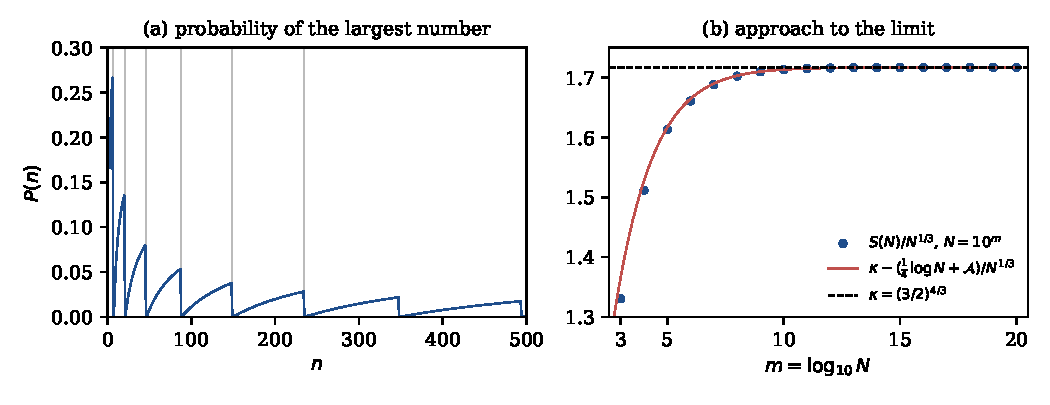
\includegraphics[width=\textwidth]{fig_equilibrium.pdf}
\caption{The game $G_n(0)$. (a) The probability $P(n)$ of the largest
number for $3\le n\le500$; the grey lines mark the zeros $n=t_k(0)-1$.
Within the positive part of each block $P$ increases. It drops to $0$
one step before the support widens. (b) $S_0(N)/N^{1/3}$ at $N=10^m$
for $3\le m\le20$ (dots), the
limit $\kappa$ (dashed), and the curve $\kappa-(\frac14\log N+\Alp)/N^{1/3}$.}
\label{fig:equilibrium}
\end{figure}

\FloatBarrier
\section{Concluding remarks}\label{sec:remarks}

The structure of the equilibria rests on two features of the payments:
they grow linearly, which makes the payoff differences in
Lemma~\ref{lem:rows} positive and the neighbour equations solvable, and
the largest payment enters only through $y=n-\frac h2$. For
$h\notin\mathcal E\cup\{0,1\}$, Remark~\ref{rem:exceptional} proves
that the thresholds eventually coincide with those of $h=0$ or $h=1$;
the proof of Theorem~\ref{thm:asymptotics} should then give the same
first-order formula, with a constant $\Alp(h)$ defined by the actual
block sums, while the term of order $1/K$ acquires an $h$-dependent part.
We have not pursued this.

We list some questions that we have not answered.
\begin{enumerate}
\item Does $\Alp$ have a closed form in classical constants? Is it
irrational?
\item Can the asymptotic definition of $\Alp(h)$ be extended to every
$h\notin\mathcal E$, and how does the resulting function depend on
$h$? The thresholds change at the points of $\mathcal E$, which
accumulate at $1$ and $2$.
\item What is the nature of the series $\sum_jb_{j,\pm}k^{-j}$ in
Table~\ref{tab:coefficients}? Its coefficients grow quickly, and we
expect it to diverge.
\item The method of Theorem~\ref{thm:asymptotics} should give further
terms of $S_h(N)$ in powers of $1/K$, with polynomial coefficients in
$\tau$. A general description of these polynomials would be
interesting.
\end{enumerate}

The exact checks of all displayed identities and examples, the
computation of the tables and the figure, and the programs that certify
$\Alp$ and $\Alp(1)$ are included in the source archive and at
\url{https://github.com/AlperTheKing/alper-constant}. AI assistance was
used in the derivations, in writing and running the verification code,
and in preparing this manuscript. Review status: Author reviewed.
The results have not been refereed or
verified in a proof assistant. This is an unrefereed preprint.

\begin{thebibliography}{9}
\small
\raggedright

\bibitem{DLMF}
NIST Digital Library of Mathematical Functions.
F.~W.~J. Olver, A.~B. Olde~Daalhuis, D.~W. Lozier, B.~I. Schneider,
R.~F. Boisvert, C.~W. Clark, B.~R. Miller, B.~V. Saunders, H.~S. Cohl
and M.~A. McClain, eds.
\url{https://dlmf.nist.gov/}.

\bibitem{ES}
EulerSolve.
\emph{Problem 1012: Rock Paper Scissors}, solution notes.
\url{https://eulersolve.org/problem/1012/} (accessed 5 October 2026).

\bibitem{PSLQ}
H.~R.~P. Ferguson, D.~H. Bailey and S.~Arno.
Analysis of PSLQ, an integer relation finding algorithm.
\emph{Math. Comp.} \textbf{68} (1999), 351--369.
\href{https://doi.org/10.1090/S0025-5718-99-00995-3}{doi:10.1090/S0025-5718-99-00995-3}.

\bibitem{FLINT}
The FLINT team.
\emph{FLINT: Fast Library for Number Theory}, and its Python interface
\emph{python-flint}.
\url{https://flintlib.org}.

\bibitem{Gosper}
R.~W. Gosper, Jr.
Decision procedure for indefinite hypergeometric summation.
\emph{Proc. Natl. Acad. Sci. USA} \textbf{75} (1978), 40--42.
\href{https://doi.org/10.1073/pnas.75.1.40}{doi:10.1073/pnas.75.1.40}.

\bibitem{Arb}
F.~Johansson.
Arb: efficient arbitrary-precision midpoint-radius interval arithmetic.
\emph{IEEE Trans. Comput.} \textbf{66} (2017), 1281--1292.
\href{https://doi.org/10.1109/TC.2017.2690633}{doi:10.1109/TC.2017.2690633}.

\bibitem{JKK}
N.~L. Johnson, A.~W. Kemp and S.~Kotz.
\emph{Univariate Discrete Distributions}, 3rd ed.
Wiley, Hoboken, 2005.

\bibitem{PE}
Project Euler.
\emph{Problem 1012: Rock Paper Scissors}.
\url{https://projecteuler.net/problem=1012} (accessed 5 October 2026).

\bibitem{vN}
J.~von Neumann.
Zur Theorie der Gesellschaftsspiele.
\emph{Math. Ann.} \textbf{100} (1928), 295--320.
\href{https://doi.org/10.1007/BF01448847}{doi:10.1007/BF01448847}.

\end{thebibliography}
\end{document}
